\chapter{Monte Carlo Methods}
\label{chap:qmc}
\todo{...}
\todo{look especially at thijssen and the foulkes review for these sections}

% probably get some inspiration from Kai's and Werner's theses -- focus on FCIQMC

\gls{MC} methods are a class of numerical methods that use random sampling to numerically solve problems. It has found applications in an impressive range of fields, from physics to finance.\todo{citation} It is particularly useful for problems with high dimensionality, where deterministic methods are often impractical. In quantum chemistry and physics, since a `dimension' can refer to any degree of freedom, high-dimensional problems are commonplace, and so \gls{MC} methods are a natural choice.

While the name \gls{MC} was coined by Stanislav Ulam, after the famous casino in Monaco,\todo{citation} the foundational concept was already developed in the 18th century by the French mathematician Georges-Louis Leclerc, Comte de Buffon. As one of the earliest example applications, in the Buffon needle problem, one can randomly toss needles onto a lined sheet of paper and determine $\pi$.\todo{citation}

\section{Classical Monte Carlo Methods}

We start our discussion with classical \gls{MC} methods. We consider the classical textbook problem of calculating the value of $\pi$, then we give it a more rigorous framework.

\subsection{A Very Bad Game of Darts}

If we imagine throwing darts at a dartboard randomly, we can approximate $\pi$. If the radius of the circle is $r$, then its area is $\pi r^2$. The area of the square circumscribing the circle is $4r^2$. Therefore, the ratio of the area of the circle to the area of the square is $\pi/4$. If we randomy sample a point in the square (``throw a dart''), the probability that the point is inside the circle is proportional its area. Since we sample inside the square, the probability of landing inside the circle is
\begin{equation}
    P(\text{inside circle}) =  \frac{\pi r^2}{4r^2} = \frac{\pi}{4}.
\end{equation}
Therefore, if we sample a large number of points, the ratio of the number of darts that land inside the unit circle to the total number of darts, we can approximate the probability distribution $P$ and thus get an estimate for $\pi$. This is illustrated in \autoref{fig:darts}, and captures the core philosophy of \gls{MC} methods.

\begin{figure}[htbp]
    \centering
    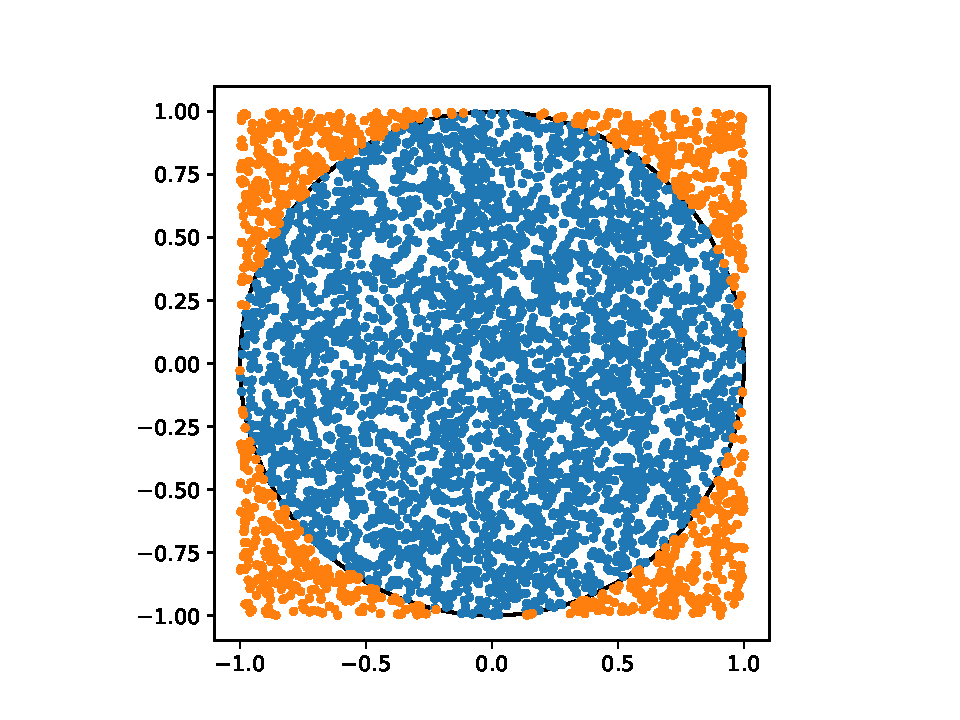
\includegraphics[width=\textwidth]{figures/qmc/darts.pdf}
    \caption{Our ``game of darts''. Points inside the unit circle are coloured blue whereas points outside are orange. Using stochastic sampling, this naive approach uses 5000 randomly generate numbers between -1 and 1 to approximate $\pi\approx 4N_\mathrm{in}/N_\mathrm{out}\approx 3.1464$. Of course, there are many ways to improve this method, the most obvious being to use a fraction of the unit circle, such as the first quadrant.}
    \label{fig:darts}
\end{figure}

\subsection{A More Mathematical Description}

\subsection{The Metropolis-Hastings Algorithm}

\section{Going Quantum: Variational Monte Carlo}
\todo{make sure to mention the Jastrow factor}

\section{Diffusion Monte Carlo}
\todo{main point here is just its similarity to FCIQMC}

\section{Auxiliary Field Quantum Monte Carlo}

\section{The Fermion Sign Problem}
\todo{make sure to mention the fixed node approximation here}

\section{QMC Meets Electronic Structure: the FCIQMC Algorithm}
\label{sec:fciqmc}

\subsection{The Sign Problem in FCIQMC}

\subsection{The Initiator Approximation}

\subsection{Reduced Density Matrix Sampling}

\subsection{Combining TC with Modern Electronic Structure}
